%(BEGIN_QUESTION)
% Copyright 2011, Tony R. Kuphaldt, released under the Creative Commons Attribution License (v 1.0)
% This means you may do almost anything with this work of mine, so long as you give me proper credit

Undersøk denne prosesstrenden, som viser responsen fra en strømningstransmitter på en 10\% trinnendring opp og ned i signalet fra regulatorutgangen (regulator satt i manuell modus) til strømningsreguleringsventilen:

$$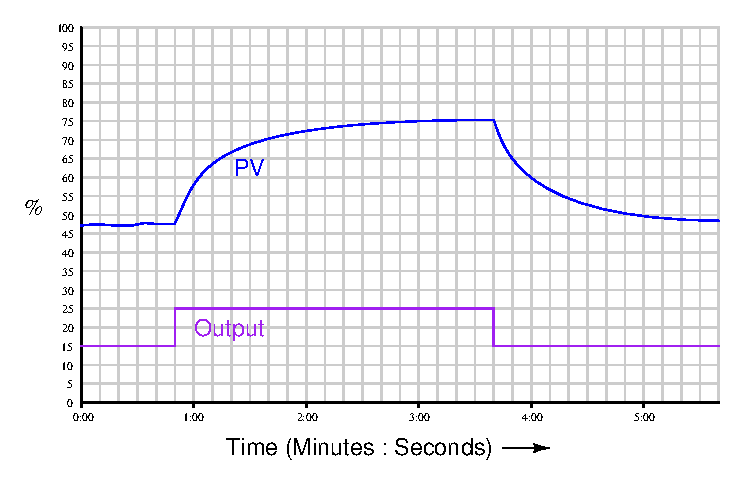
\includegraphics[width=15.5cm]{i01654x01.eps}$$

To teknikere har undersøkt denne trenden og diskuterer årsaken til den trege responsen. Den ene sier at det sannsynligvis skyldes en transmitter med for mye filtrering (demping) programmert inn. Den andre sier at det er en treg reguleringsventil. Begge forklaringer er plausible.

\vskip 10pt

Lag en entydig test som kan bekrefte eller avkrefte disse hypotesene.

\vfil

\underbar{file i01654}
\eject
%(END_QUESTION)





%(BEGIN_ANSWER)

Dette er et vurdert spørsmål -- ingen svar eller hint er gitt!

%(END_ANSWER)





%(BEGIN_NOTES)

Det grunnleggende problemet vi står overfor her, er hvordan vi skal skille om transmitteren eller ventilen er ansvarlig for den etterslepende trenden, siden begge kan gi samme trendbilde. For å løse dette må vi finne en annen informasjonskilde (noe annet enn trendgrafen).

\vskip 10pt

En løsning er å gå til ventilen og inspisere den fysisk mens den får trinnendringen i utgangssignal! Hvis ventilresponsen visuelt er treg (dvs. ikke raskt går til ny posisjon når den får en trinnkommando i regulatorutgangen), ligger problemet i ventilen. Hvis responsen er kvikk, ligger problemet i transmitteren (eller at regulatoren er konfigurert med for mye filtrering).

\vskip 10pt

En tredje mulighet, som teknikerne ikke nevnte i oppgaven, er filtrering i regulatorinngangen. En diagnostisk test for dette er å måle inngangssignalet med multimeter eller loopkalibrator (satt til å ``lese'' strøm) mens trinnendringstesten utføres på nytt. Hvis signalresponsen er kvikk, ligger problemet i filtrering i regulatoren; hvis signalresponsen fortsatt er kraftig dempet, ligger problemet i transmitteren eller i ventilen.

En fjerde mulighet er at strømningstransmitteren er DP-basert og har delvis tett impulsledning mellom DP-transmitteren og strømningsorganet (f.eks. orificeplate, venturi eller pitotrør). En delvis tett impulsledning vil dempe responsen på plutselige trykkendringer omtrent på samme måte som førsteordens elektronisk filtrering.

%INDEX% Process troubleshooting: diagnosing problem via trend recording

%(END_NOTES)
